\documentclass[10pt,twocolumn,letterpaper]{article}

\usepackage{iccv}
\usepackage{times}
\usepackage{epsfig}

\usepackage{graphicx}
\graphicspath{{figures/}}

\usepackage{amsmath}
\usepackage{amssymb}
\usepackage{color}
\usepackage{caption}
\usepackage{subcaption}
\usepackage{multirow}
\usepackage{bbm}


% \usepackage{titlesec}
\newcounter{example}%[section]
\renewcommand{\theexample}{\arabic{example}}
\newenvironment{example}{
        \vspace{1.5ex}
        \refstepcounter{example}
        {\noindent\bf Example \theexample:}}{
        \eop\vspace{1.5ex}}


\newcommand{\eat}[1]{}
\newcommand{\kw}[1]{{\ensuremath {\mathsf{#1}}}\xspace}
\newcommand{\eop}{\hspace*{\fill}\mbox{$\Box$}}
\newcommand{\kwlog}{\emph{w.l.o.g.}\xspace}
\newcommand{\stitle}[1]{\vspace{1.5ex}\noindent{\bf #1}}
\newcommand{\etitle}[1]{\vspace{0.8ex}\noindent{\underline{\em #1}}}
\newcommand{\aka}{\emph{a.k.a.}\xspace}
\newcommand{\gpmm}{\kw{GPM}}
\newcommand{\vqa}{\kw{VQA}}
\newcommand{\nlq}{Q_{nl}}
\newcommand{\eag}{G_{EA}}


% Include other packages here, before hyperref.

% If you comment hyperref and then uncomment it, you should delete
% egpaper.aux before re-running latex.  (Or just hit 'q' on the first latex
% run, let it finish, and you should be clear).
\usepackage[pagebackref=true,breaklinks=true,letterpaper=true,colorlinks,bookmarks=false]{hyperref}

% \iccvfinalcopy % *** Uncomment this line for the final submission

\def\iccvPaperID{****} % *** Enter the ICCV Paper ID here
\def\httilde{\mbox{\tt\raisebox{-.5ex}{\symbol{126}}}}

% Pages are numbered in submission mode, and unnumbered in camera-ready
\ificcvfinal\pagestyle{empty}\fi
\begin{document}

%%%%%%%%% TITLE
\title{Visual Question Answering with Graph Matching and Reasoning}

\author{First Author\\
Institution1\\
Institution1 address\\
{\tt\small firstauthor@i1.org}
% For a paper whose authors are all at the same institution,
% omit the following lines up until the closing ``}''.
% Additional authors and addresses can be added with ``\and'',
% just like the second author.
% To save space, use either the email address or home page, not both
\and
Second Author\\
Institution2\\
First line of institution2 address\\
{\tt\small secondauthor@i2.org}
}

\maketitle
%\thispagestyle{empty}


%%%%%%%%% ABSTRACT
\begin{abstract}
Visual Question Answering (\vqa) is of great significance in offering people convenience: one can raise a question for details of objects, or high-level understanding about the scene, over an image. 
This paper proposes a novel method to address the \vqa problem. In contrast to prior works, our method that targets single scene \vqa, replies on graph-based techniques and involves reasoning. In a nutshell, our approach is centered on three graphs. The first graph, referred to as inference graph $G_I$, is constructed via learning over labeled data. The other two graphs, referred to as query graph $Q$ and entity-attribute graph $\eag$, are generated from natural language query $\nlq$ and image {\cal I}mg, that are issued from users, respectively. As $\eag$ often does not take sufficient information to answer $Q$, we develop techniques to infer missing information of $\eag$ with $G_I$. Based on $\eag$ and $Q$, we provide techniques to find matches of $Q$ in $\eag$, as the answer of $\nlq$ in {\cal I}mg. Unlike commonly used 
\vqa methods that are based on end-to-end neural networks, our graph-based method shows well-designed reasoning capability, and thus is highly interpretable. We also create a dataset on soccer match (Soccer-VQA) with rich annotations. The experimental results show that our approach outperforms the state-of-the-art method and has high potential for future investigation.
\end{abstract}


%%%%%%%%% BODY TEXT
% unchanged
\section{Introduction}
\label{sec-intro}

In recent years, visual question answering (\vqa) has received significant attention~\cite{malinowski2015ask,ren2015image,gao2015you} as it involves multi-disciplinary research, \eg natural language understanding, visual information retrieving and multi-modal reasoning. The task of \vqa is to find an answer to a question $\nlq$ based on the content of an image. There are a variety of applications of \vqa, \eg surveillance video understanding, visual commentator robot, \etc. Solving \vqa problems usually requires high level reasoning from the content of an image.

\begin{figure}[tb]
\centering
\includegraphics[width=\columnwidth]{motivation.eps}
\caption{The image is about soccer match, where each person object is associated with attributes: id, uniform color, status (\underline{S}tanding, \underline{M}oving, \underline{E}xpansion), direction (\underline{B}acking, \underline{F}acing, \underline{N/A}), as well as location, and the soccer object is attributed with location. %Part (b) shows a part of corresponding entity-attribute graph. Part (c) exhibits a $\nlq$ and its corresponding query graph $Q$. 
}
\vspace{-4ex}
\label{fig:example}
\end{figure}


\begin{example}
Figure~\ref{fig:example} depicts an image about a soccer match, where two teams are distinguished by red and green uniforms, and each object is associated with a set of attributes. A typical query may ask ``How many players are there in the image?''. Though simple, it is a challenging task to efficiently answer the query, since (1) it is often very inefficient to detect all the objects in the given image, following traditional way, while only query related objects are in demand; (2) one not only needs to identify all the {\em person} objects, but also have to infer their hidden attribute ``role'', which is often ambitious. 

Motivated by these, one may analyze questions first and detects only those objects as well as their attributes that are in connection with questions, then infer missing values of hidden attributes, and answer questions. In this way, not only query accuracy but also query efficiency are expected to be guaranteed.  
\end{example}


This example suggests that we leverage adaptive query understanding and reasoning to address the \vqa problem. While to do this, two critical questions have to be answered. (1) How to understand queries and carry query-related visual tasks? (2) How to infer crucial information to assist query answering?  


\vspace{2ex}
\stitle{Contributions.} In contrast to a majority of deep learning based \vqa techniques, which not only overlooks correlation between queries and images, but also lacks of necessary reasoning, we propose a novel technique that integrates adaptive query understanding and reasoning.  The main contributions of the paper are as follow.  

(1) We model images and queries as graphs, and propose to answer visual queries with graph matching. This new representation and answering scheme constitute the base of our techniques.  

(2) We introduce a method to guide visual tasks based on reinforcement learning. That is, given an image and a question, our method can identify a set of visual tasks that are question related, and direct subsequent visual processing in a more efficient manner. 

(3) We propose approaches to answering visual queries based on reasoning and graph matching. More specifically, we first transform a given image into an entity-attribute graph; we then develop method to infer missing value for question answering; %As verified in our empirical studies, the classifier is very effective, with accuracy reaching X\%. 
we finally show how to answer queries with graph matching. %To this end, we first transform a natural language query into a pattern query, and then employ matching technique to find answers. 

4) We conduct extensive experimental studies to verify the performance of our method. We find that X, Y, and Z. 

% change one paragraph
\section{Related Work}
\label{sec-related-work}
\hspace{-2ex}
%Traditional approaches to the \vqa problem are mainly neural network based. In contrast, our approach consists of query understanding, query oriented object detection, and query answering. 
We categorize related work into following three parts. %: visual query answering, visual objects, and graph-based query answering. %\looseness=-1


\etitle{Visual query answering}. Current \vqa approaches are mainly based on deep neural works.  \cite{zhu2016visual7w} introduces a spatial attention mechanism similar to the model for image captioning. %In this method, a weight vector is computed and served as an additional input at each time step of the LSTM model. 
Instead of computing the attention vector iteratively, \cite{xu2016ask} obtains a global spatial attention weights vector which is then used to generate a new image embedding. \cite{zhu2017structured} proposed to model the visual attention as a multivariate distribution over a grid-structured conditional random field on image regions, thus multiple regions can be selected at the same time. This attention mechanism is called structured multivariate attention in~\cite{zhu2017structured}.
There has been many other improvements to the standard deep learning method, \eg %compared to element-wise product or concatenation of the visual and textual representations,
\cite{fukui2016multimodal} utilized Multimodal Compact Bilinear (MCB) pooling to efficiently and expressively combine multimodal features. Another interesting idea is the implementation of Neural Module Networks~\cite{Andreas_2016,hu2017learning}, which decomposes queries into their linguistic substructures, and uses these structures to dynamically instantiate module networks. %Question-specific deep network is then assembled from these module networks that each solve one subtask. The layout of module networks can either be constructed from off-the-shelf parses~\cite{Andreas_2016}, or learned from the data~\cite{hu2017learning}.
\cite{teney2017graph} proposed to build graph over scene objects and question words. The visual graph is similar to ours, but the query graph differs. %\cite{teney2017graph} exploits the grammatical relations between words to generate query graph, while our method applies directed acyclic graph to represent query sentence. 
Note that the method \cite{teney2017graph} proposed is still a neural network based method as the structured representations are fed into a recurrent network to form the final embedding and the answer is again inferred by a classifier. %In contrast to recent works~\cite{Lu2015, Lu2016Hie}, we focus on single scene and involve reasoning. 


\etitle{Environment Exploration in Visual Field}. Reinforcement driven information acquisition is not only focusing at games~\cite{NIPS2017_7084,NIPS2002_2171,NIPS2017_7007} but also wildly applied in traditional vision domain.~\cite{DBLP:conf/cvpr/MathePS16} implement reinforcement learning in visual object detection, by presenting a novel sequential
models which accumulate evidence collected at a small set of
image locations to detect visual objects effectively.~\cite{DBLP:conf/cvpr/GoodrichA12} forms the facial detection problem into an adaptive learning process, by designing an approximate optimal control framework, based on reinforcement learning to actively search a visual field.~\cite{DBLP:conf/nips/MnihHGK14} introduced a novel recurrent neural network model which is capable to extract information from an image or video by adaptive selection for a sequence of regions or locations.~\cite{zhu2017icra} introduced reinforcement learning in the task of target-driven visual navigation. Other works aims to achieving based on algorithms~\cite{5596468,DBLP:conf/aaai/AbtahiF11}.

In visual and language domain, relevant work like~\cite{DBLP:conf/cvpr/RenWZLL17} achieves image captioning with Embedding Reward. Reinforcement learning preserves ability to effectively select preferred actions, which benefits the system decomposing the problem into a few sub-tasks.


\eat{%20190305
{Visual Objects Processing}. Visual object detection as well as relationship identification are the preliminary tasks for not only \vqa but also image captioning~\cite{lu2016visual,yao2018exploring,teney2017graph}. %Many works in not in VQA but in image captioning has been done by firstly detect the visual objects~\cite{lu2016visual,yao2018exploring}, and then discover the relationship among them. 
Other works, \eg~\cite{yao2017boosting}, produce high-level attributes for input images, based on which further processing can be conducted. %These will help model to have a better understanding on properties of different regions/objects. 
These prior works show that detecting all visual objects, their attributes and relationships is very vital for resolving \vqa problem. %However, these work do not consider the relationship in detail, moreover it is quite hard to demonstrate spatial relationship (\eg close and far) and get relative distance between objects, due to perspective front view of the image.
%Even though, we  these techniques do not exactly solve the same problem as us, we get inspiration from them that, to explore the relationship between objects or image regions, we first need to detect all visual objects along with relevant attributes.
}%20190305


\etitle{Graph-based \vqa}. ~\cite{TuMLCZ14} proposes a framework to understand events and answer user queries, where underlying knowledge is represented by a spatial-temporal-causal And-Or graph (S/T/C-AOG). (Neural-Symbolic \vqa) recovers a structural scene symbolization from the image which is similar to graph representation, and learns a program trace from the question, which is later executed on the scene representation to obtain the answer. Our method differs in the way of answer retrieval by graph matching instead of program execution, furthermore, our method incorporates an inference graph to infer the missing values which turns out to improve the performance significantly. [] (FVQA) conducts question-query mapping and then query-KB matching which is most similar to our method. Our model is different from [] in that we implement reinforcement learning to make both visual processing and query generation more efficiently. Another strength of our method, again, is the introduction of inference graph which leads to powerful reasoning capability.

\eat{%20190318
Query answering has been extensively studied for graph data. In a nutshell, this work includes two aspects: query understanding, and query evaluation. We next review previous work on two aspects. 

\noindent (1) Queries expressed with natural languages are very user-friendly, but nontrivial to understand. Typically, they need to be structured before issuing over \eg search engine, knowledge graph, since structured queries are more expressive. There exist a host of works that based on query logs, human interaction and neural network, respectively. \cite{PoundHIW12} leverages query logs to train a classifier, based on which structured queries are generated.  \cite{ZhengC0YZ17} propose an approach to generate the structured queries through talking between the data (\ie the knowledge graph) and the user. \cite{YihCHG15} introduced how to generate a core inferential chain from a query with convolutional neural networks. As we only cope with a set of fixed queries, hence, we defer
the topic of query understanding to another paper, and focus primarily on the query evaluation. \looseness=-1

\noindent (2) To evaluate queries on graphs, a typical method is graph pattern matching. There has been a host of work
on graph pattern matching, \eg techniques for finding exact matches~\cite{cordella2004sub-full,subiso76}, inexact matches~\cite{ZouCO09,TianP08}, and evaluating \kw{SPARQL} queries on \kw{RDF} data~\cite{WagnerTLHS12}. Our work differs from the prior work in the following: (1) we integrate arithmetical and set operations in the query graph, and (2) we develop technique to infer missing values for query answering. \looseness=-1
}%20190318

% \subsection{Outline of the Paper}

% The rest of the paper is organized as follows. Section ~\ref{Preliminary} reviews notions and notations used in the paper. Section~\ref{sec-overview} outlines the framework our approach. Section \ref{sec-understanding} presents core components of our approach, \ie $\kw{VA}$ module (Section ~\ref{Visual Object}), inference module $\kw{IGC}$ (Section ~\ref{Inference}) and $\kw{GM}$ module (Section ~\ref{Query Answering}). Section ~\ref{Experiments} presents our experiments, followed by conclusion in Section ~\ref{Conclusion}.


% unchanged
\section{Overview of the Approach}
\label{sec-overview}

%%%%%%%%%%%%%%%
\begin{figure*}[tb!]
\vspace{-1ex}
\centerline{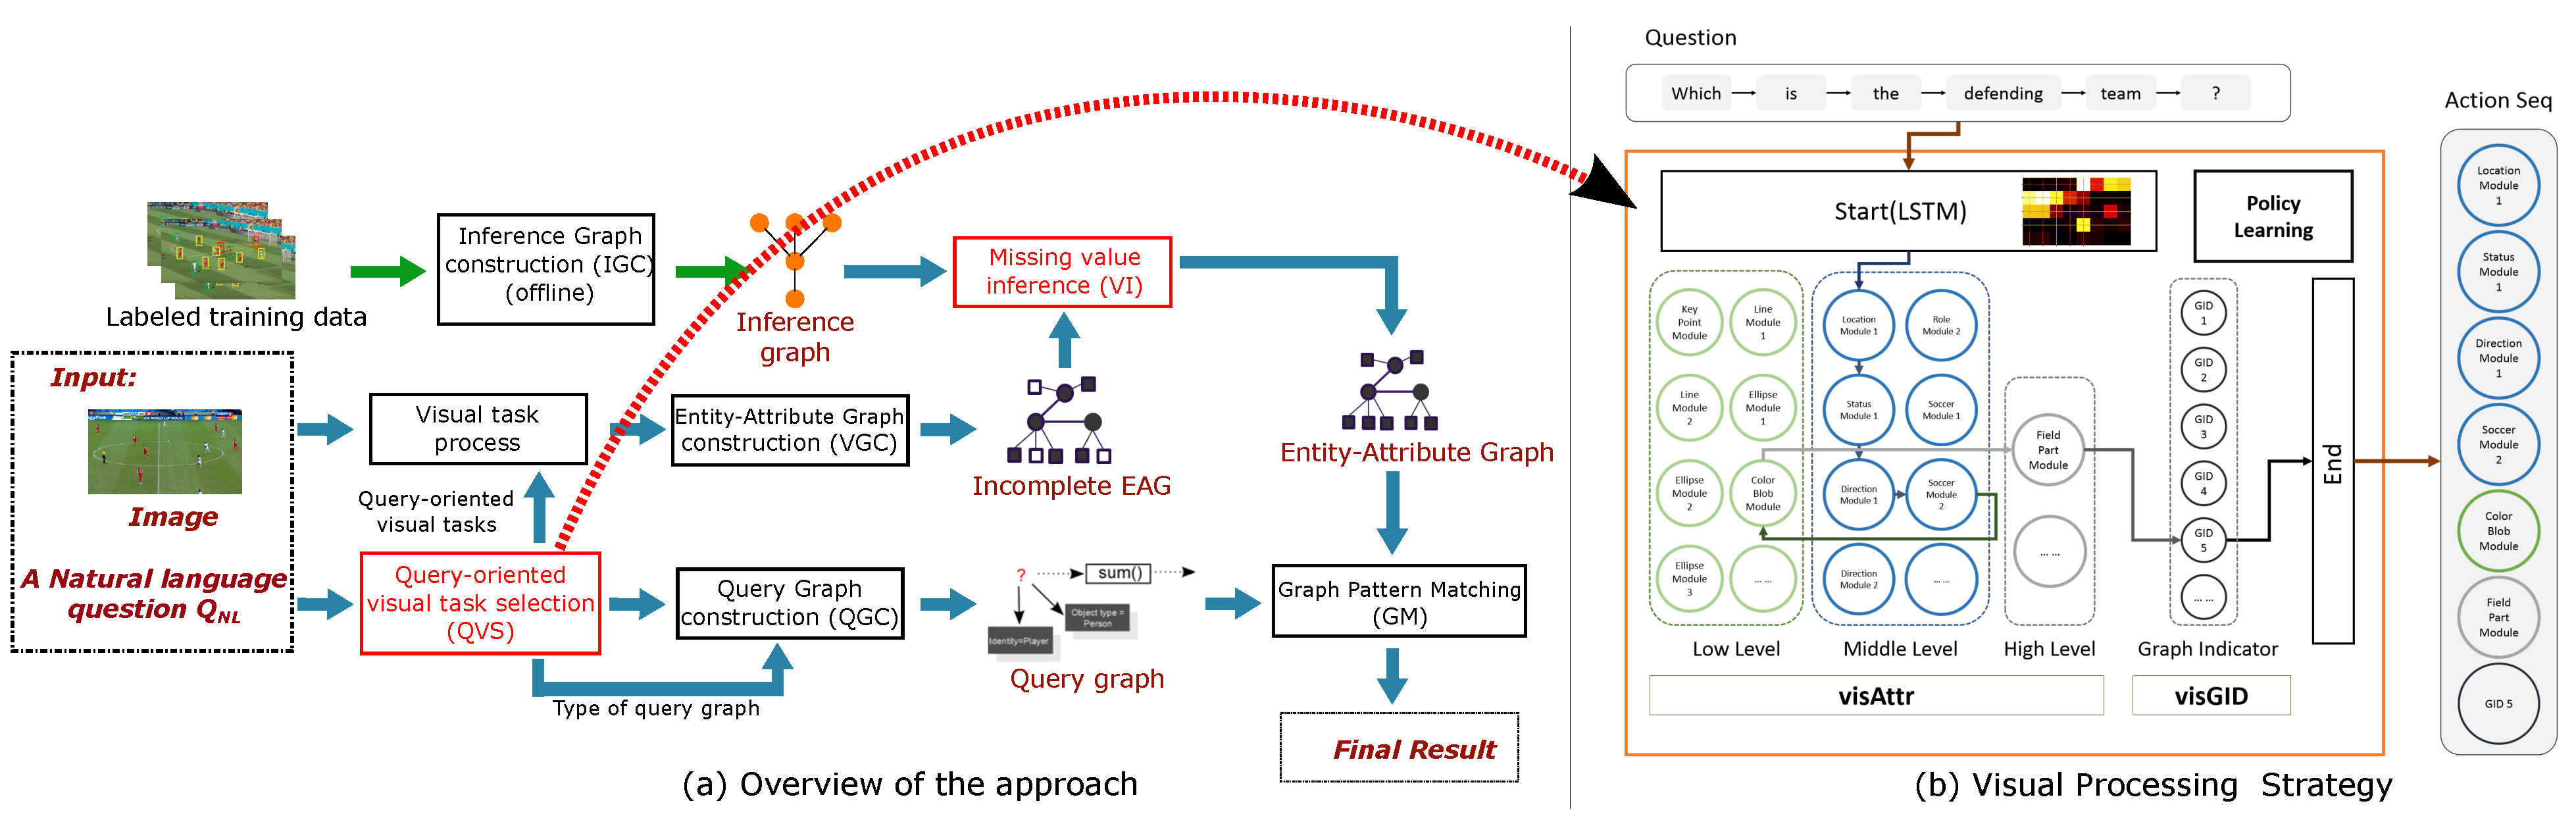
\includegraphics[scale=0.28]{overview.eps}}
\caption{Overview of our approach, and graph-based representation of images and questions} \label{fig-overview}
\vspace{-2ex}
\end{figure*}
%%%%%%%%%%%%%%%%

We start from representations of images and questions, followed by the overview of our approach.


\subsection{Representation of Images and Questions}
\label{sec-representation}

We use the same representations as~\cite{peixi2019}. To make the paper self-contained, we cite them as follows (rephrased). 

\stitle{Entity-Attribute Graphs.} Entities are typically defined as objects or concepts that exist in the real world. An entity often carries attributes, that describe features of the entity. \looseness=-1

Assume a set ${\cal E}$ of entities, a set ${\cal D}$ of values, a set ${\cal P}$ of predicates indicating attributes of entities and a set $\Theta$ of types. 
Each entity $e$ in ${\cal E}$ has a {\em unique ID} and a {\em type} in $\Theta$.

An {\em entity-attribute} graph, denoted as \kw{EAG}, is a set of triples $t = (s, p, o)$, where {\em subject} $s$ is an entity in ${\cal E}$, $p$ is a {\em predicate} in ${\cal P}$, and {\em object} $o$ is either an entity in ${\cal E}$ or a value $d$ in ${\cal D}$. It can be represented as a directed edge-labeled graph $\eag=(V, E)$, such that (a) $V$ is the set of nodes consisting of $s$ and $o$ for each triple $t = (s, p, o)$; and (b) there is an edge in $E$ from $s$ to $o$ labeled by $p$ for each triple $t = (s, p, o)$. \looseness=-1


\eat{%20190305
We consider two types of equality:

\noindent (a) {\em node identity} on ${\cal E}$: $e_1\Leftrightarrow e_2$ if entities $e_1$ and $e_2$ have the same ID, \ie they refer to the same entity; and 

\noindent (b) {\em value equality} on ${\cal D}$: $d_1 = d_2$ if they are the same value.

In $\eag$, $e_1$ and $e_2$ are represented as the same node if $e_1\Leftrightarrow e_2$; 
similarly for values $d_1$ and $d_2$ if $d_1=d_2$.
}%20190305


An image can be represented as an \kw{EAG} with detected objects along with their detected attributes, and relationships among objects. This can be achieved via a few visual tasks. While \kw{EAG} generated directly after image processing is often incomplete, \ie it may miss some crucial information to answer queries. We hence refer to {\em entity-attribute graphs} with incomplete information as {\em incomplete entity-attribute graphs}, and associate nodes with white rectangles, to indicate the missing value of an entity or attribute in \kw{EAG}. Figure~\ref{fig:example}(b) is an {\em incomplete entity-attribute graph}, in which square nodes representing person roles are associated with white rectangle. 

\stitle{Query Graphs.}  A query graph $Q(u_o)$ is a set of triples
$(s_Q, p_Q, o_Q)$, where $s_Q$ is either a variable $z$ or a function $f(z)$ taking $z$ as parameter, $o_Q$ is one of a value $d$ or $z$ or $f(z)$, and $p_Q$ is a predicate in ${\cal P}$. Here function $f(z)$ is defined by users, and variable $z$ has one
of three forms: (a) {\em entity variable} $y$, to map to an entity, (b)
{\em value variable} $y*$, to map to a value, and (c) {\em wildcard} $\_y$, to
map to an entity. Here $s_Q$ can be either $y$ or $\_y$, while $o_Q$ can
be $y$, $y*$ or $\_y$. Entity variables and wildcard carry a {\em type},
denoting the type of entities they represent. 

A query graph can also be represented as a graph such
that two variables are represented as the same node if they
have the same name of $y$, $y*$ or $\_y$; similarly for functions $f(z)$ and values $d$.
We assume \kwlog that $Q(x)$ is connected, \ie there exists
an undirected path between $u_o$ and each node in $Q(u_o)$.
In particular, $u_o$ is a designated node in $Q(u_o)$, denoting the query focus and labeled by ``?''. %denoting an entity. Introduce functions.  \looseness=-1
Take Fig.~\ref{fig-overview}(c) as example. It depicts a query graph that is generated from query ``{\em How many players are there in the image?}''. Note that the ``query focus'' $u_o$ carries a function \kw{num}() that calculates the total number of {\em person} entities with {\em role} ``player''. 


\subsection{Approach Overview}
\label{sec-architecture}

% %%%%%%%%%%%%%%%
% \begin{figure*}[tb!]
% \vspace{-1ex}
% \centerline{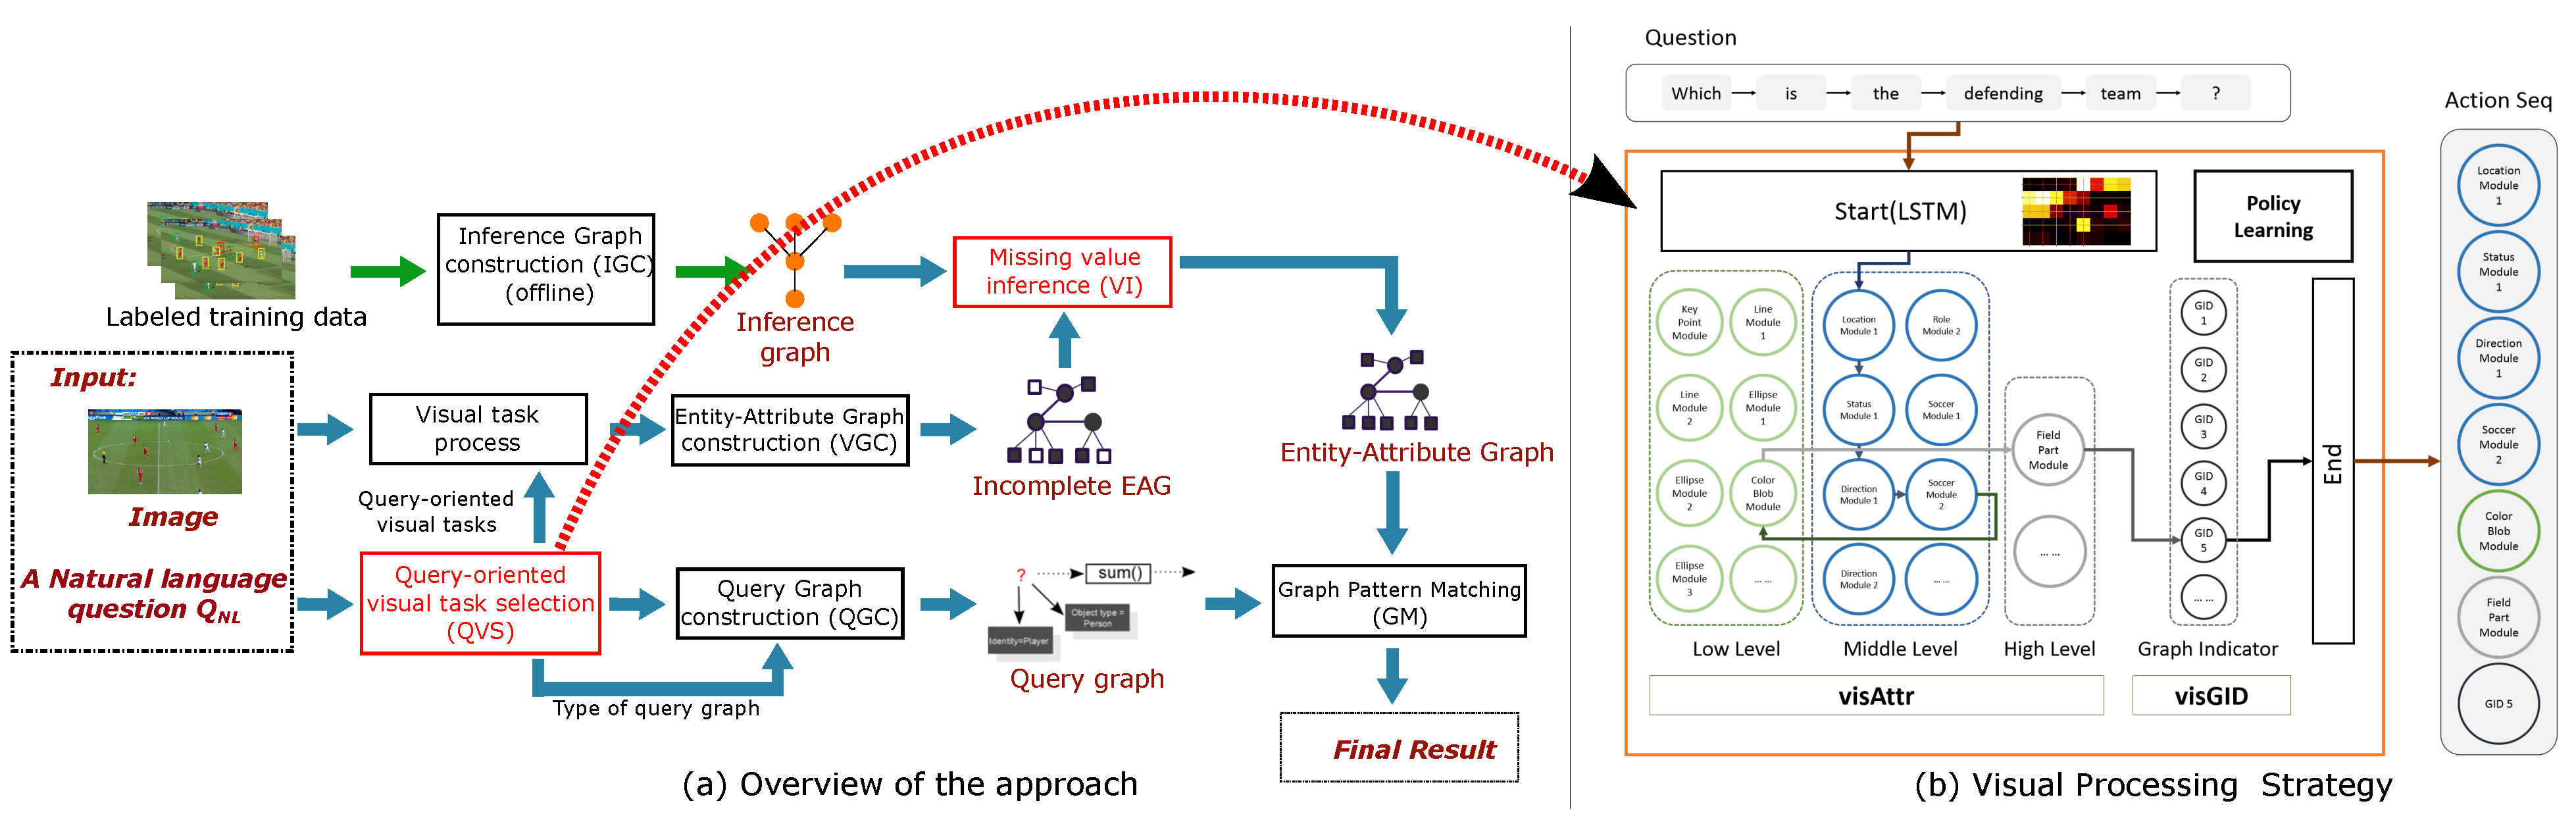
\includegraphics[scale=0.28]{overview.eps}}
% \caption{Overview of our approach, Entity Attribute Graph and Queries} \label{fig-overview}
% \vspace{-2ex}
% \end{figure*}
% %%%%%%%%%%%%%%%%


\eat{
Along the same lines as representations for images and questions, and graph pattern matching for question answering, raised in~\cite{peixi2019}, we propose a comprehensive approach as modeling of the \vqa problem. %answer a set of typical questions regarding soccer matches. 
}

Figure~\ref{fig-overview}(a) presents the overview of our approach. In a nutshell, our approach copes with two types of computations, \ie online computation, which responses to user's questions and offline computation that trains inference graphs (\ie a classifier) for missing value inference. 

For online computation, our approach leverages five modules, \ie 


Specifically, our approach consists of two types of 

As can be seen, our approach revolves around three graphs: entity-attribute graph, query graph and inference graph. The generation of entity-attribute graph $\eag$ follows three steps. Module \kw{VA} conducts the first step, \ie image processing, and outputs all the detected objects along with their attributes. Using visual contents produced in step one, module \kw{VGA} constructs an {\em incomplete} \kw{EAG}. In the last step, module \kw{VI} takes inference graph and {\em incomplete} \kw{EAG} as inputs, infer missing information with $G_I$, and outputs an updated \kw{EAG} for query answering. 
The inference graph $G_I$ is used to infer missing values of an {\em incomplete} $\kw{EAG}$. %In $G_I$, each node either denotes an attribute of an object or a class label indicating the class of the object, and each edge represents assignment of attribute value (resp. class label). $G_I$ is 
and constructed by module \kw{IGC} over training data. As is query-independent, $G_I$ is constructed offline, which warrants the efficiency of our approach. %The other two graphs \ie entity-attribute graph and query graph are produced in parallel. 
As the other part of input, natural language query $\nlq$ needs to be structured for query evaluation. To this end, $Q_{NL}$ is first parsed via our \kw{NLP} module, and then structured by module \kw{QGC}. After $Q(u_o)$ and $\eag$ are generated, our approach employs module $\kw{GM}$ for matching computation, and returns final result. \looseness=-1 %When extra information is required to answer the query, we use leverage a knowledge graph $\kw{KG}$ to provide additional information. \kw{KG} can be constructed offline via existing mature methods. 


It takes an image and a natural language question $Q_{NL}$ as input, and works as following. (1)


As some modules employ existing techniques, to emphasize our novelty, we will elaborate modules $\kw{VA}$ and $\kw{VGA}$ in Section~\ref{sec-understanding}, modules \kw{IGC} and \kw{VI} in Section~\ref{Inference}, and module \kw{GM} in Section~\ref{Query Answering} with more details. \looseness=-1

% changed
\section{Query Oriented Visual Tasks}
\label{sec-reinforcement-learning}
In this section, we introduce how we do visual tasks that are in connection with questions. 


\subsection{Visual Processing}
\label{sec-visual-processing}
\begin{figure}[h]
\begin{center}
\includegraphics[width=\linewidth]{RLplot.pdf}
\end{center}
\caption{Overview of our approach}
\label{fig:RLplot}
\end{figure}

In our approach, we build a structure which selects sub-tasks to form a policy which is based on queries. For instance, with the input \textit{which is the defending team?}, the system first predicts the corresponding visual action sequence, which are \textit{Human Module}, \textit{Gesture Module}, \textit{Direction Module}, \textit{Soccer Module}, \textit{Color Blob Module}, \textit{Field Part Module} and \textit{Graph Indicator}. Guided by such sequence, the image features are then extracted by operating relevant vision tasks. An overview is shown in Figure~\ref{fig:RLplot}.


\subsubsection{Multi-layer LSTM with Attention}
\label{sec-LSTM}
\hspace{\parindent}The task here is to predict the most suitable action modules sequence $\kw{a}$ by given questions $Q$ and preference $pre$. We form the problem of seeking effective answering strategy of question $Q$ and preference $pre$ as a sequence-to-sequence learning problem with attention mechanism. Inspired by~\cite{Bahdanau2016}, we input word feature of questions $w_i^q$, $i\in\|Q\|$ into a LSTM network which is regarded as an encoder and output $h_i$ as the hidden state for $i$th word in the question. By adding soft attention, the context vector $c_i$ is calculated by the following equations.


\begin{small}
\begin{equation} 
    c_i= \sum\nolimits_{j=1}^{\|Q\|} a_{ij}h_{ij}
\end{equation}
\begin{equation} 
    a_{ij}= \frac{exp(e_{ij})}{\sum\nolimits_{k=1}^{\|Q\|} exp(e_{ik})}
\end{equation}
\begin{equation} 
    e_{ij}= a(s_{j-1},h_i)
\end{equation}
\end{small}

\noindent where $h_i$ and $s_j$ are hidden states of encoder and decoder stage, respectively. Here $a_{ij}$ is the attention weights, with higher $a_{ij}$ in $(i, j)$ pair, the more attention will pay in this correlation, thus the $j$th output action $\kw{a}_i$ module will be more influenced by the $i$th input word $w_i^q$ in question. The decode part is similar as traditional recurrent neural networks (RNN). The following steps demonstrates decoding to get the joint distribution of action module sequence $\kw{A} = [\kw{a}_1,\dots,\kw{a}_t]$.

\begin{small}
\begin{equation} 
    p(\kw{A}|Q) = \Pi_{t\in\|\kw{A}\|}~p(\kw{a}_t|\{\kw{a}_1,\dots,\kw{a}_t\},c_i,Q)
\end{equation}
\begin{equation} 
    p(\kw{a}_t|\{\kw{a}_1,\dots,\kw{a}_t\},c_i,Q)= g(\kw{a}_{t-1},s_t,c_i,Q)
\end{equation}
\begin{equation} 
    s_t = f(s_{t-1},\kw{a}_{t-1},c_i)
\end{equation}
\end{small}
\noindent where $g(\cdot)$ is a nonlinear function which outputs the probability of action module \kw{a_{t}}. The probability distribution $p(\kw{A}|Q)$ is used to predict a maximum probability action module sequence by beam search during testing time.

Guided by this action sequence $[\kw{a}_1,\kw{a}_2,\kw{a}_3,\dots,\kw{a}_n]$, actions are selected from the following visual task pool, and comes into next session, visual task selection (\kw{VTS}).


\subsubsection{Visual Task Selection}
\label{sec-VTS}
\hspace{\parindent}\kw{VTS} is guided by the question feature, selecting target visual tasks from the visual task pool by Monte Carlo learning. The task pool is demonstrated in Table~\ref{table:visual_tasks}.


\begin{table}[th]
\centering \scriptsize
\begin{tabular}{|l|ll|l|}
\hline
visAttr & \multicolumn{1}{l|}{Level}  & Sub-task           & Descriptions                                                                                                                                 \\ \cline{2-4} 
        & \multicolumn{1}{l|}{Low}    & Keypoint Module    & \multirow{3}{*}{\begin{tabular}[c]{@{}l@{}}To get detailed information of the \\ soccer field $F_{keypoint}$.\end{tabular}}                  \\ \cline{3-3}
        & \multicolumn{1}{l|}{}       & Line Module        &                                                                                                                                              \\ \cline{3-3}
        & \multicolumn{1}{l|}{}       & Ellipse Module     &                                                                                                                                              \\ \cline{3-4} 
        & \multicolumn{1}{l|}{}       & Color Blob Module  & \begin{tabular}[c]{@{}l@{}}To detect blobs of different colors \\ among a region(whole soccer \\ field or a small bounding box).\end{tabular} \\ \cline{2-4} 
        & \multicolumn{1}{l|}{Middle} & Location Module    & \begin{tabular}[c]{@{}l@{}}To detect the location of the \\ person $P_{location}$.\end{tabular}                                              \\ \cline{3-4} 
        & \multicolumn{1}{l|}{}       & Status Module      & \begin{tabular}[c]{@{}l@{}}To get the person's gesture \\ $P_{status}$ (standing, moving, \\ expansion).\end{tabular}                        \\ \cline{3-4} 
        & \multicolumn{1}{l|}{}       & Direction Module   & \begin{tabular}[c]{@{}l@{}}To get whether a person is facing \\ the goal or not $P_{direction}$.\end{tabular}                               \\ \cline{3-4} 
        & \multicolumn{1}{l|}{}       & Uniform Module     & \begin{tabular}[c]{@{}l@{}}To get the uniform color of the \\ person $P_{uniform}$.\end{tabular}                                              \\ \cline{3-4} 
        & \multicolumn{1}{l|}{}       & Soccer Module      & \begin{tabular}[c]{@{}l@{}}To detect the location of the \\ soccer $S_{location}$.\end{tabular}                                              \\ \cline{2-4} 
        & \multicolumn{1}{l|}{High}   & Field Part Module  & \begin{tabular}[c]{@{}l@{}}To detect which part of the\\ soccer field is there in the \\ image $F_{part}$ .\end{tabular}                     \\ \hline
visGID  &                             & Graph ID Indicator & \begin{tabular}[c]{@{}l@{}}To indicate which type of graph\\ will be used in the following \\process.\end{tabular}                          \\ \hline
\end{tabular}
\caption{Visual Task Pool}
\label{table:visual_tasks}
\end{table}


The pool is constructed by two parts, the first one is \textit{visAttr} which aims to discover the attribute of people, soccer, field and scene~\cite{peixi2019}, while the other one \textit{visGId} is an indicator showing the current question belongs to which graph type. There are three levels of \textit{visAttr}: low, middle and high, which represents different difficulty degree of the vision tasks. 

\begin{figure}[thb]
\centering
        \begin{subfigure}[b]{0.088\textwidth}
                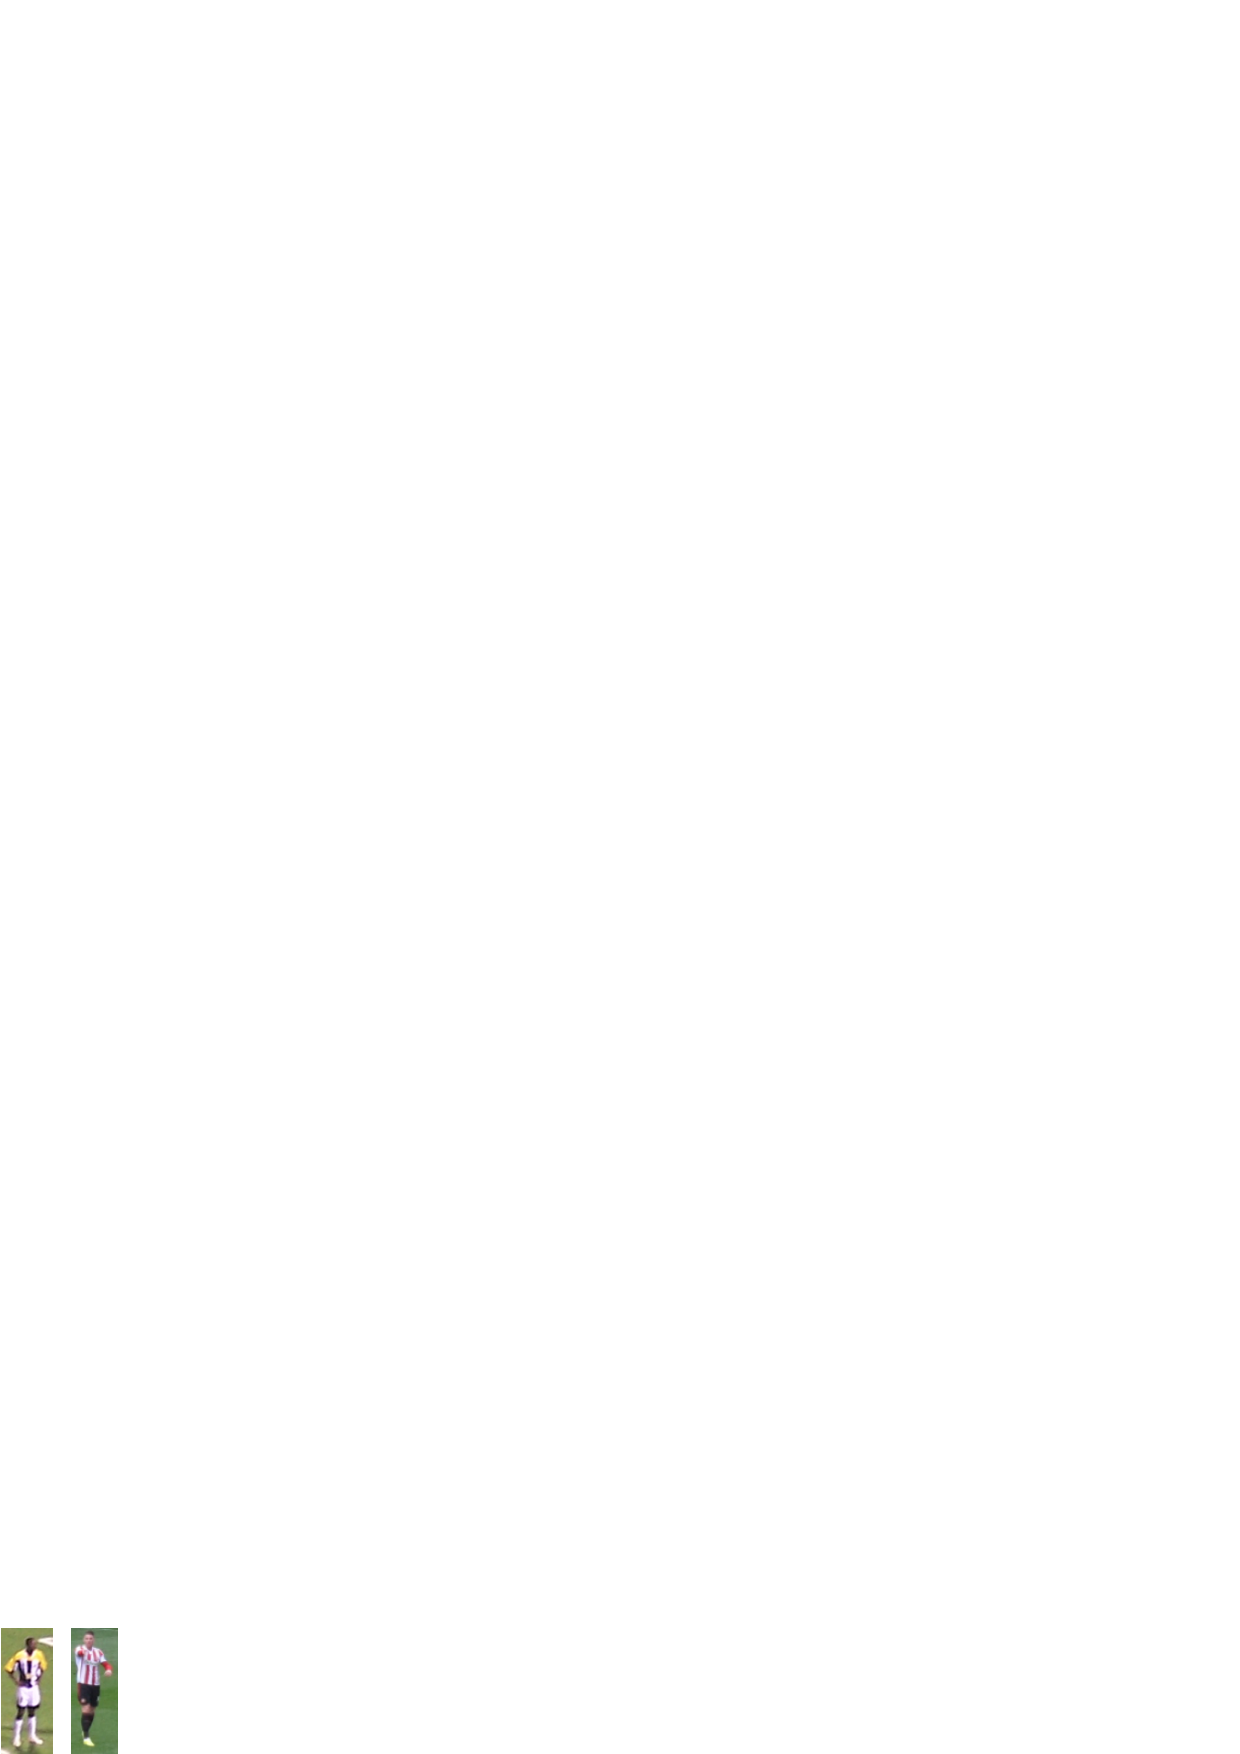
\includegraphics[width=\linewidth]{stand1.png}
                \caption{Standing}
                \label{fig:gull}
        \end{subfigure}\quad
        \begin{subfigure}[b]{0.127\textwidth}
                
\includegraphics[width=\linewidth]{move1.png}
                \caption{Moving}
                \label{fig:gull2}
        \end{subfigure}\quad
        \begin{subfigure}[b]{0.166\textwidth}
                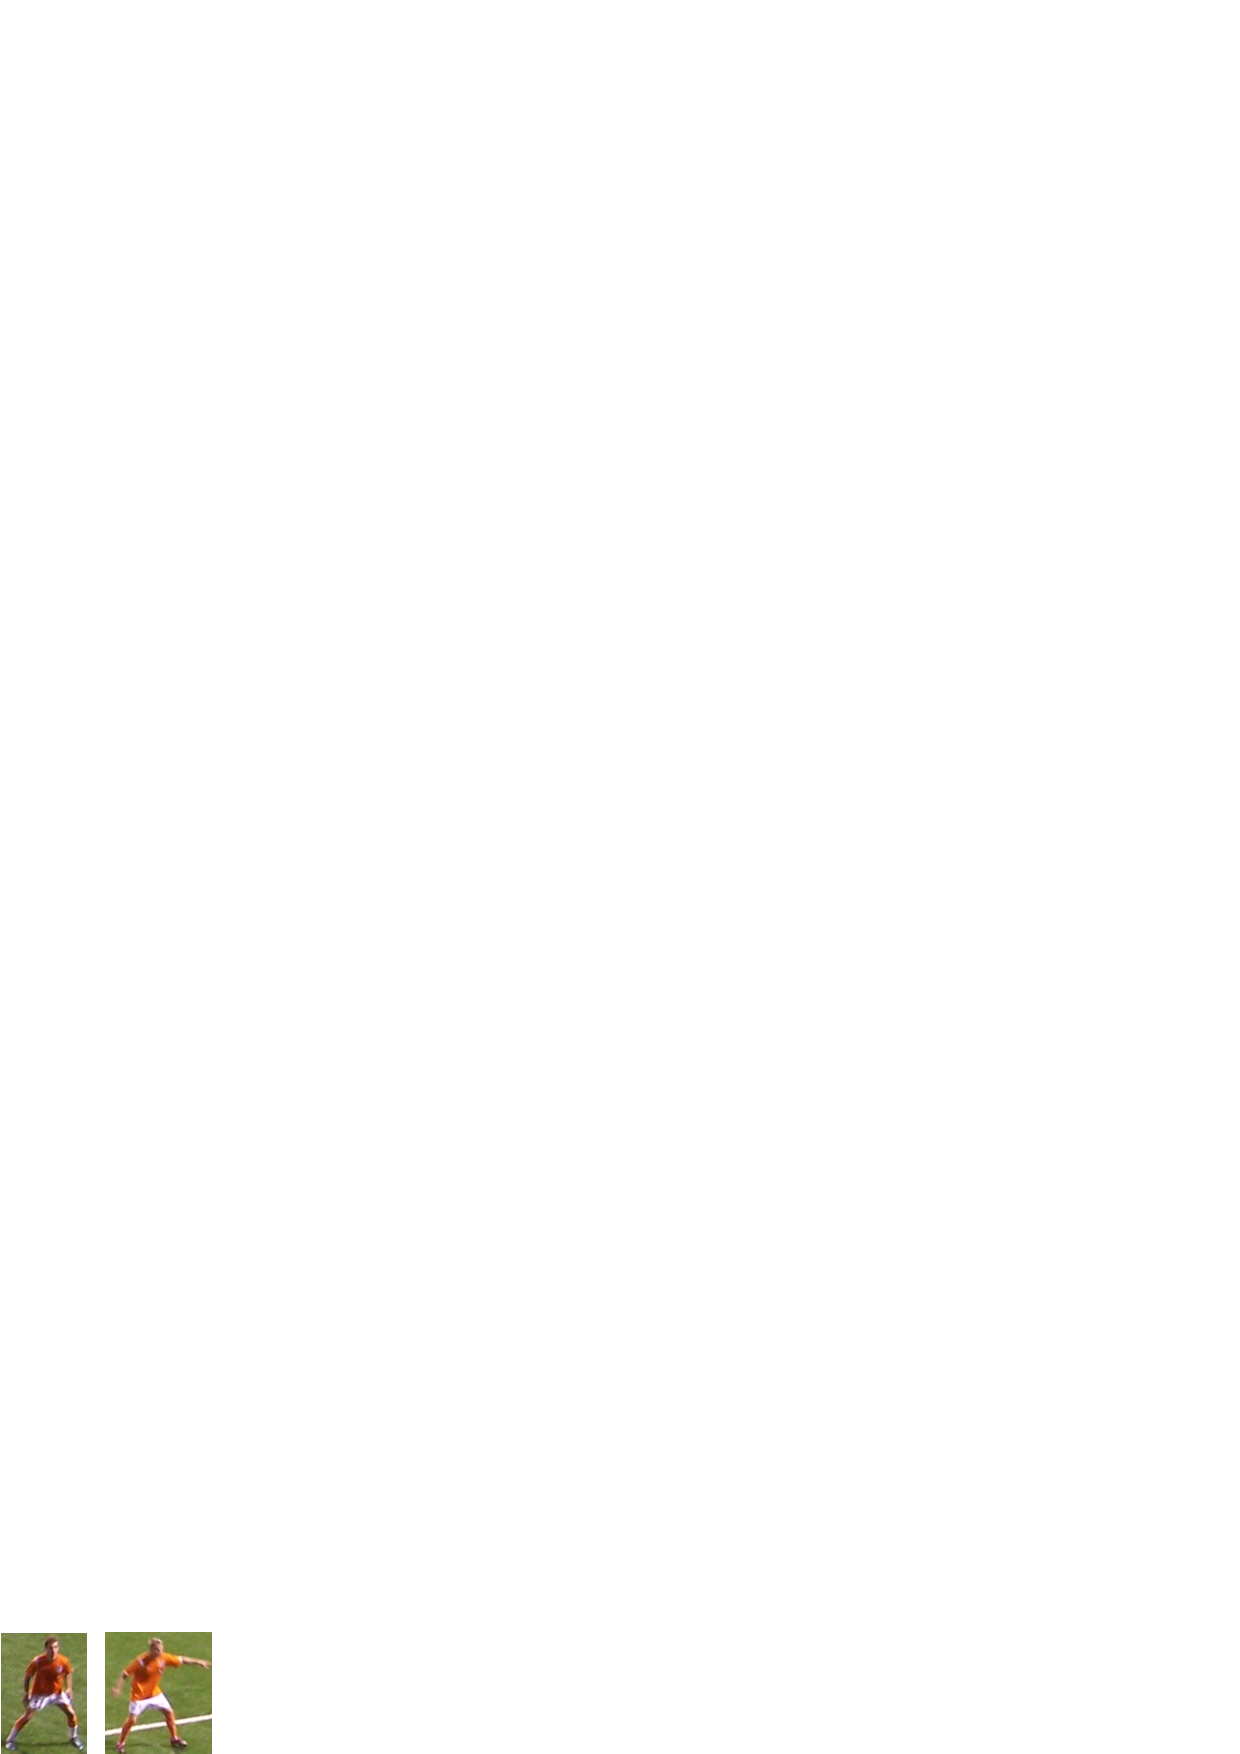
\includegraphics[width=\linewidth]{expand1.png}
                \caption{Expansion}
                \label{fig:tiger}
        \end{subfigure}
        \caption{Person status.}\label{fig:Person Status}
\end{figure}

For each vision task, the approach is not fixed, one task can be achieved by different methods with variance in time and accuracy. For instance, object detection based methods, like Faster R-CNN~\cite{Ren:2015:FRT:2969239.2969250}, R-FCN~\cite{DBLP:conf/nips/DaiLHS16}, SSD~\cite{DBLP:conf/eccv/LiuAESRFB16} or skeleton keypoints detection based method like~\cite{cao2017realtime} and~\cite{wei2016cpm} can be implemented as a set of status module methods, because all of them is able to localize and distinguish people who are moving, standing or with an expansion gesture (Figure~\ref{fig:Person Status}). Thus, the system is not only able to determine whether resembles a vision task module into action module sequence $[\kw{a}_1,\kw{a}_2,\kw{a}_3,\dots,\kw{a}_n]$, it can also select one specific approach under a vision task module, based on question and preference. For the preference, it is clarified in the next section.


\subsubsection{Time and Accuracy Term}
\label{sec-TimeAcc}
\hspace{\parindent} To better balance the accuracy and inference time for a given application, we proposed time and accuracy terms in loss function during training process.

\begin{small}
\begin{equation} 
    L_{\tau\alpha}(\theta) = \ell(\theta,\kw{A}|I, Q) + \gamma\sum_{i\in\|\kw{A}\|}\alpha(\kw{a_i}) + (1-\gamma)\sum_{i\in\|\kw{A}\|}\tau(\kw{a_i})
\end{equation}
\end{small}

\noindent where $\tau(\cdot)$ and $\alpha(\cdot)$represent the pre-tested inference time and inference accuracy, action module sequence \kw{A} samples from joint distribution $p(\kw{A}|Q)$, and here $\ell(\cdot)$ is the softmax loss over the predict score. For the preference term $\gamma$, it ranges from 0 to 1, which represents the preference over time and accuracy.

\subsubsection{Monte Carlo Methods}
\label{sec-MC}
\hspace{\parindent} The task now becomes a policy learning problem. Given a question and preference, output a policy containing a sequence of actions $[\kw{a}_1,\kw{a}_2,\kw{a}_3,\dots,\kw{a}_n]$. There is no ground truth for each steps, but only a final reward indicates that whether the answer is correct based on current policy. We involve the concept of Monte Carlo Methods to learn the policy which guides the vision tasks, and such policy network requires an extra reward value in loss.

\begin{small}
\begin{equation} 
    L_{policy}(\theta) = \sum\nolimits_{i\in\|A\|} log\pi(\kw{a}_{i}|Q,\theta)\ell(Q,\kw{A})
\end{equation}
\end{small}

\noindent where \kw{a_{i}} is the action will take, based on current status. $\pi(\cdot)$ is the policy function that maps status to actions, here, the policy is the probability of outputing next action module $\kw{a_{i}}$ based on current status. And $\ell(\cdot)$ here is the softmax loss based on the whole action module sequence $[\kw{a}_1,\kw{a}_2,\kw{a}_3,\dots,\kw{a}_n]$. Since all actions are discrete, which leads to non-differentiable, and back-propagation cannot be used. Policy gradient~\cite{Liu_2017_ICCV} is used here during training. The object function now becomes the combination of policy gradient loss $L_{policy}(\theta)$ with the time-accuracy-balanced loss $L_{\tau\alpha}$, and optimize it by backpropagation for $L_{\tau\alpha}$, while policy gradient for $L_{policy}(\theta)$.


\subsection{Construction of \kw{EAG}}
\label{sec-eag-construction}

After objects that are related to questions are identified, we construct a graph structure, denoted as \kw{EAG}, along the same line as~\cite{peixi2019}. 


\begin{example}
\label{exm-x1}
ADD AN EXAMPLE TO ILLUSTRATE PROGRESS IF NECESSARY!
\end{example}


% changed
\section{Reasoning}
\label{sec-reasoning}

According to our observation,  an {\em incomplete} \kw{EAG} isn't well satisfying of answering the query because of the insufficient attributes.
To infer the hidden attributes, 
%In our proposed method, 
an inference graph is constructed accordingly.  
we briefly introduce the construction below. 

\subsection{Construction of Inference Graph}
To take advantage of the prior information and increase the generalization ability of the proposed model, our inference graph is constructed using Bayesian network.
Mathematically, Bayesian network \cite{friedman1997bayesian} can be described by a pair $\mathfrak{B}=<\mathcal{G},\varTheta_\mathcal{G}>$. 
Here, the notation $\mathcal{G}$ is a directed acyclic graph, of which the $i$-th vertex corresponds to a random variable $X_i$, and the edge between two connected vertexes indicates the dependency. 
Additionally, the second item $\varTheta_\mathcal{G}$ is a set of parameters used to quantify the dependencies in $\mathcal{G}$.
Denoted by $\text{Pa}(X_i)$ the attributes of the parents of $X_i$, 
the parameter of $X_i$ is represented by  $\theta_{X_i | \text{Pa}(X_i)} = P_\mathfrak{B}(X_i| \text{Pa}{(X_i)})$.
%We use the notation $\theta_{X_i | \text{Pa}(X_i)} = P_\mathfrak{B}(X_i| \text{Pa}{(X_i)})$ to denote the parameter of $X_i$, of which $\text{Pa}(X_i)$ is the attributes of the parents of $X_i$.
With the notations above, the joint probability distribution of Bayesian network is given by:

\begin{equation}\label{eq:BNOri}
P_\mathfrak{B}(X_1, \cdots, X_n) = 
\prod_{i=1}^{n} P_\mathfrak{B}(X_i| \text{Pa}{(X_i)})=
\prod_{i=1}^{n} \theta_{X_i | \text{Pa}(X_i)}
%\theta_{x_1|\text{Pa}_1(\mathbf{x})}\theta_{x_2|\text{Pa}_2(\mathbf{x})}\cdots \theta_{x_n|\text{Pa}_n(\mathbf{x})}
\end{equation}
\vspace{-1ex}

In our inference graph, the role of Bayesian network is to predict the object class when given the attributes $\{X_i\}_{i=1}^n$ as input. In the sense of probability, the object class is also a variable \cite{koller2009probabilistic}.
Defined by $X_0=Y$ the class variable, the network now has one extra vertex $X_0$.
In order to infer the class attribute, and according to the Bayesian rule, our problem becomes:

\vspace{-1ex}
\begin{align}\label{eq:BNWithCls}
\begin{split}
P_\mathfrak{B}(Y|{X}) & = 
\frac{ P_\mathfrak{B}(Y) P_\mathfrak{B}({X}|Y) }{P_\mathfrak{B}({X})}\\
&=\frac{ \theta_{Y|\text{Pa}({X}_0)} \prod_{i=1}^{n} \theta_{X_i|Y, \text{Pa}({X}_i)} }{ \sum_{y'\in \mathcal{Y}} \theta_{y'|\text{Pa}({X}_0)} \prod_{i=1}^{n} \theta_{X_i|y', \text{Pa}({X}_i)} }
\end{split}
\end{align}
where $\mathcal{Y}$ is the set of classes.

%\begin{figure}[tb]
%\centering
%\includegraphics[width=\columnwidth]{inferGraphWorkflow}
%\caption{The pipeline of inference graph used for inferring the role of a person object.}
%\vspace{-4ex}
%\label{fig:inferGraphWorkflow}
%\end{figure}

\subsection{Learning the Structure of Inference Graph}

In the context of Na\"{i}ve Bayes, 
the structure of $P_\mathfrak{B}(Y|{X})$ is simplified by taking the class variable as the root, and all attributes are conditionally independent when taking the class as a condition \cite{petitjean2018accurate}. As a consequence, the attribute class can be explicitly inferred by:

\begin{equation}\label{eq:BN-naiveBayes}
P_\mathfrak{B}(Y| {X}) = c \cdot \theta_Y \prod_{i=1}^{n}\theta_{X_i|Y}
\end{equation}
where $c$ is a scale factor that makes the calculation being a distribution: $c=\sum_{y'\in \mathcal{Y}}  \theta_{y'} \prod_{i=1}^{n}\theta_{X_i|y'}$.

Note from Eq.\eqref{eq:BN-naiveBayes} that Na\"{i}ve Bayes simplifies the complexity of Bayesian network. As can be validated by the experimental results, the simple model works excellently to our problem. 

%\begin{figure}[tb!]
%\centering
%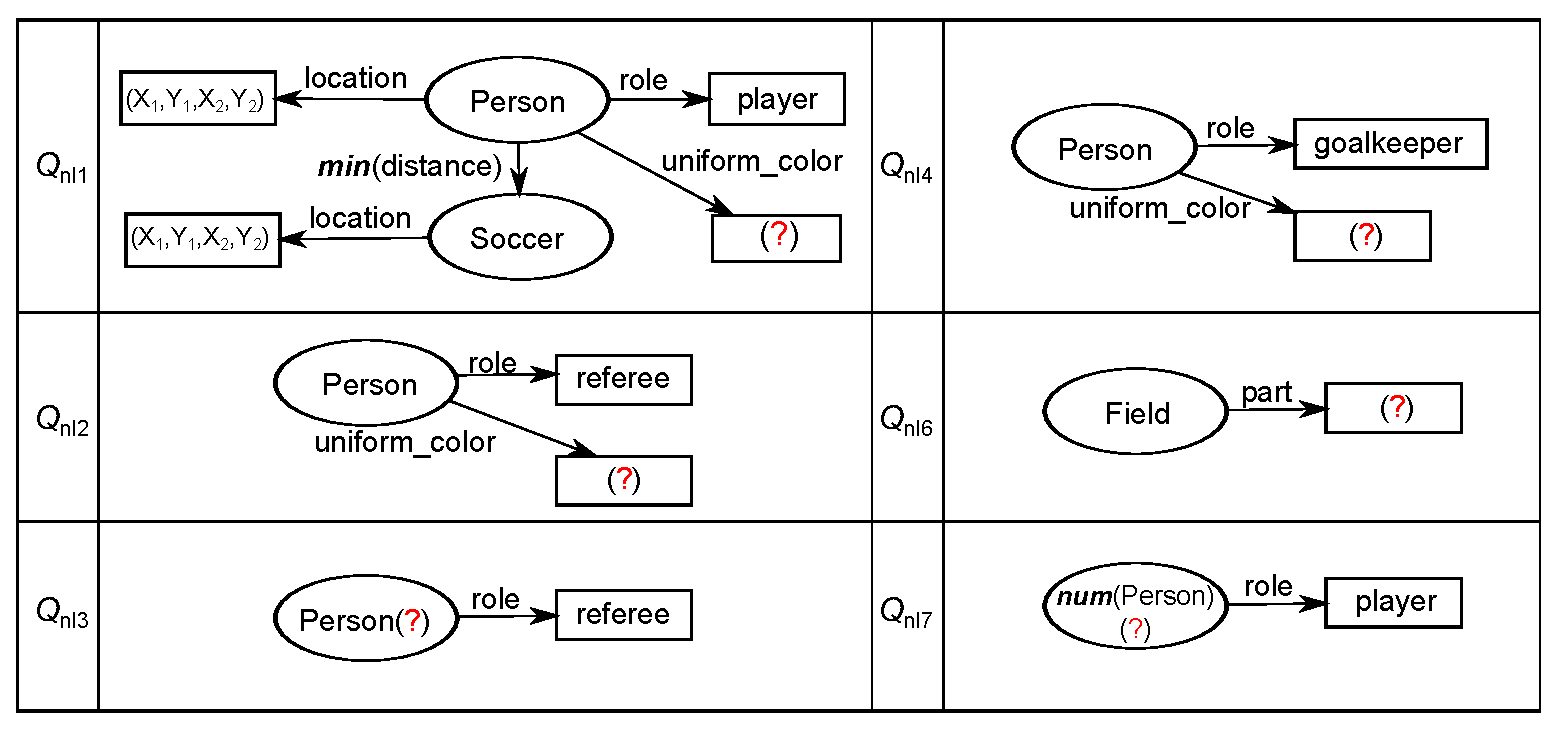
\includegraphics[width=\columnwidth]{queries.eps}
%\caption{Query graphs}
%\label{fig:queries}
%\end{figure}

% small change
\section{Experimental Studies}
\label{sec-expt}

In this section, we conducted two sets of experiments to evaluate (1) the performance of our visual processing module, (2) the accuracy of our inference module, and (3) the overall performance of our approach. 

\stitle{Experimental Setting}. %We report settings of experimental studies. 

\etitle{DataSet}. We used two datasets: (1) \kw{Soccer} dataset that we annotated; and (2) X dataset from~\cite{}. We extracted images with subjects of golf and tennis (report Statistics about the dataset). We split \kw{Soccer} (resp. X) data into two parts:{\em  I} (one third) and {\em II} (two thirds), and used {\em II} as training data, and {\em I} as testing data. 

\etitle{Queries}. We used two sets of questions: (1) the set of questions given in Table~\ref{table:questions} for \kw{Soccer} dataset; and (2) another set of questions listed in Table~\ref{} for X dataset. 

\begin{table}[thb] 
\footnotesize
\begin{tabular}{|l|l|l|}
\hline
Id & Question                                           & Difficulty \\ \hline
%$Q_{nl_1}$  & Who is this image about?                         & Hard       \\ \hline
$Q_{nl_1}$  & Who is holding the soccer?                         & Easy       \\ \hline
$Q_{nl_2}$  & What is the uniform color of the referee?           & Easy       \\ \hline
$Q_{nl_3}$  & Is there any referee in the image?                 & Easy       \\ \hline
$Q_{nl_4}$  & Which team does the goalkeeper belong to?          & Medium       \\ \hline
$Q_{nl_5}$  & Who is the defending team?                         & Medium       \\ \hline
$Q_{nl_6}$  & Which part of the field are the players being now? & Hard       \\ \hline
$Q_{nl_7}$  & How many players are there in the image?           & Hard     \\ \hline
$Q_{nl_8}$  &            &      \\ \hline
$Q_{nl_9}$  &            &      \\ \hline
$Q_{nl_10}$  &            &      \\ \hline
\end{tabular} 
\caption{A set of questions} \label{table:questions}
\end{table}




\subsection{Performance of Visual Processing}

{\color{red} Peixi, please report your results with details here.}



\begin{figure}[tb!]
\centering
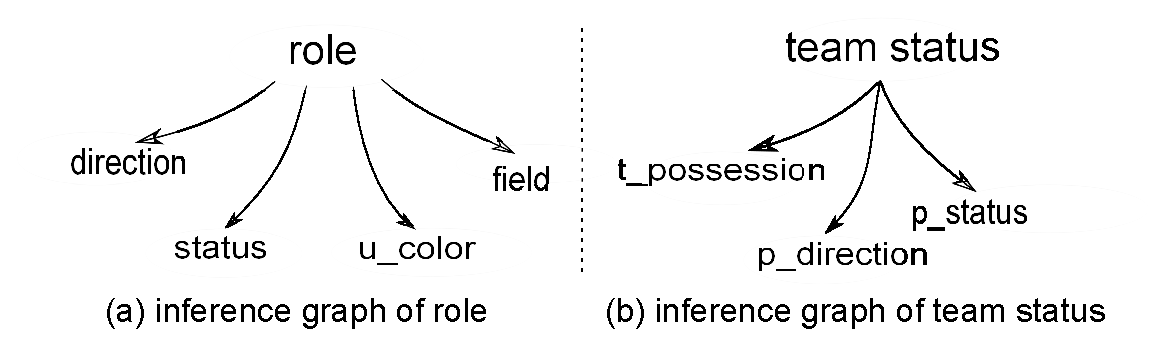
\includegraphics[width=\columnwidth]{PredictNB.eps}
\vspace{-2ex}
\caption{Inference Graphs}
\vspace{-2ex}
\label{fig:inferG}
\end{figure}

\subsection{Effectiveness of Inference} 

\stitle{Accuracy of Role}. Only report results with Reinforcement learning 

\stitle{Accuracy of Team-Status}. Only report results with Reinforcement learning 

\stitle{Accuracy of Kick-Off}. {\color{red} SHOW INFERENCE GRAPH AND RESULT TABLE!}

\stitle{Accuracy of Penalty Kick}. {\color{red} SHOW INFERENCE GRAPH AND RESULT TABLE!}

\stitle{Accuracy of Corner Kick}. {\color{red} SHOW INFERENCE GRAPH AND RESULT TABLE!}

\stitle{Accuracy of Attacking Free Kick}. {\color{red} SHOW INFERENCE GRAPH AND RESULT TABLE!}

\stitle{Accuracy of Balls}. {\color{red} Over new dataset. SHOW INFERENCE GRAPH AND RESULT TABLE!}

\subsection{Overall Performance}
\label{sec-overall-performance}

We compared the following state-of-the-art methods: X1, X2 and X3 with ours. 



{\small
\bibliographystyle{ieee}
\bibliography{egbib}
}

\end{document}
